\section{Theorie}
\label{sec:Theorie}

\subsection{Gedämpfte Schwingungen des RLC-Kreises}
Ein RLC-Kreis besteht aus einer Spule, einen Kondensator und einem Widerstand. Wird von außen
dem System Enerige zugeführt, pendelt diese zwischen dem Kondensator und der Spule hin und her.
Wegen dem Widerstand wird die Enerige mit fortlaufender Zeit in Wärme umgewandelt. Das System beschreibt
somit eine gedämpfte Schwingung.

\begin{figure}[H]
  \centering
  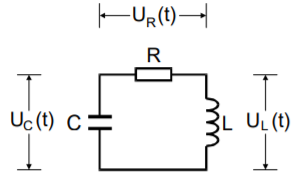
\includegraphics[height=5cm]{RLC-Kreis(Grundsaetzlich).PNG}
  \caption{Darstellung eines RLC-Kreises}
  \label{fig:RLC-Kreis(mit Widerstand)}
\end{figure}

Nach dem 2. Kirchhoff'schen Gesetz kann man die einzelnen Spannungen addieren und daraus eine Differentialgleichung
für die gedämpfte Schwingung erhalten.
\begin{align}
  U_R(t) + U_C(t) + U_L(t) = RI(t) +\frac{Q(t)}{C} + L\frac{\symup{d}I(t)}{\symup{d}t} = 0 \\
  \Rightarrow \frac{\symup{d}^2I(t)}{\symup{d}t^2} +\frac{R}{L}\frac{\symup{d}I(t)}{\symup{d}t} + \frac{1}{LC}I(t) = 0
\end{align}

Die Lösung der Differetialgleichung lautet:
\begin{align}
  &I(t) = e^{-2\pi \nu t} \left(A_1 e^{2j\pi \mu t} + A_2 e^{-2j\pi \nu t}\right)   \\
\text{mit} \:\:\:\:  &\mu = \frac{R_{eff}}{4\pi L} , \\
  &\nu = \frac{1}{2\pi} \sqrt{\frac{1}{LC} - \frac{R^2}{4L^2}} \notag.
\end{align}

Dabei ist $j$ die imaginäre Zahl.

Zwei Fälle werden unterschieden.
1. Fall: Ist $\nu$ reell gilt für $I(t)$:
\begin{equation}
  I(t) = A_0 e^{2\pi \mu t} \cos{2\pi \nu t + \eta}.
\end{equation}
Die Amplitude dieser gedämpften Schwingung geht für größer werdende $t$ gegen $0$ und die
Abklingdauer der Schwingung beträgt:
\begin{equation}
  T_{ex} =\frac{1}{2\pi \mu} = \frac{2L}{R}
\end{equation}

\begin{figure}[H]
  \centering
  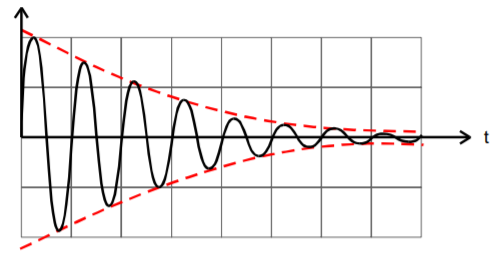
\includegraphics[height=5cm]{schwingfall.PNG}
  \caption{Darstellung des Schwingfalles einer gedämpften Schwingung mit Einhüllende $\pm e^{-2\pi \mu t}$}
  \label{fig:schwingfall}
\end{figure}

2. Fall: Ist $\nu$ imaginär enthält $I(t)$ keinen oszillatorischen Anteil mehr und es kommt
zu Relaxationserscheinungen. Je nach Wahl von $A_1$ und $A_2$ kann es zu einem Extremwert kommen, bis
$I(t)$ für große Zeiten gegen Null geht.

\begin{figure}[H]
  \centering
  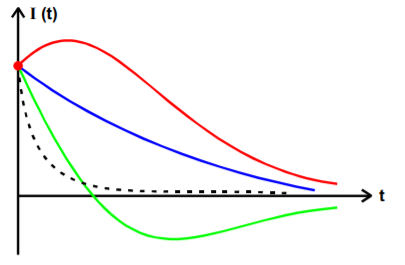
\includegraphics[height=5cm]{grenzfall.PNG}
  \caption{Zeitverläufe des Stromes bei einer aperiodischen Dämpfung (Imaginäres $\nu$)}
  \label{fig:grenzfall}
\end{figure}

Die gestrichelte Linie in Abbildung 3 zeigt den aperiodischen Grenzfall und beschreibt den Verlauf
in dem $I(t)$ am schnellsten gegen Null geht. Er tritt ein wenn $\frac{1}{LC}=\frac{R_{ap}^2}{4L^2}$ gilt, also $\nu = 0$ ist.


\subsection{Erzwungene Schwingung im RLC-Kreis}
\begin{figure}[H]
  \centering
  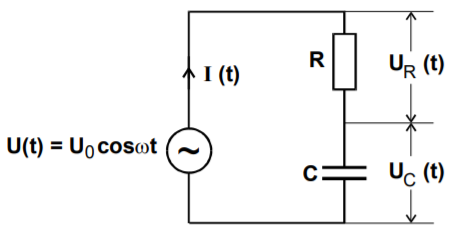
\includegraphics[height=5cm]{wechselspannung.PNG}
  \caption{RLC-Kreis mit sinusförmiger Wechselspannung}
  \label{fig:wechselspannung}
\end{figure}

Liegt an einem RLC-Kreis eine periodische Spannung $U(t) = U_0 e^{j\omega t}$ an, dann wird die Schwingung durch folgende
Differentialgleichung beschrieben:
\begin{align}
  LC\frac{\symup{d^2}U_C}{\symup{d}t^2} + RC\frac{\symup{d}U_C}{\symup{d}t} + U_C = U_0 e^{j\omega t}.
\end{align}

Aus der Differentialgleichung folgt für $U_C$
\begin{equation}
  U_C(\omega) = \frac{U_0}{\sqrt{\left(1-LC\omega^2 \right)^2 + \omega^2 R^2 C^2}} \label{eqn:U_C}
\end{equation}
Gleichung \eqref{eqn:U_C} beschreibt die Spannungsamplitude in Abhängigkeit von der Frequenz. Für große Frequenzen
geht $U_C$ gegen Null und für kleine Frequenzen gegen $U_0$.

Aus der Differentialgleichung folgt ebenfalls die Phasenverschiebung zur Erregerspannung:
\begin{equation}
  \phi (\omega) = \arctan{\left(\frac{-\omega R C}{1 - LC \omega^2}\right)}
\end{equation}
Für größer werdende Frequenzen wächst die Phasenverschiebung bis $\frac{\pi}{2}$ an.

Die Kondensatorspannung hat ein Maximum bei der Resonanzfrequenz $\omega_{res}$:
\begin{equation}
  \omega_{res} = \sqrt{\frac{1}{LC} - \frac{R^2}{2L^2}}.
\end{equation}

Für den Fall der schwachen Dämpfung $\left(\frac{R^2}{2L^2} - \ll \frac{1}{LC}\right)$ beträgt das
Spannungsmaximum:
\begin{equation}
  U_{C,max} = \frac{1}{\omega_0 RC} \cdot U_0 = qU_0.
\end{equation}

Dabei beschreibt $q$ die Güte des Schwingkreises.
%Für $R \rightarrow \infty$ wird $U_{C,max}$ unendlich groß und es kommt zur Resonanzkatastrophe.
Die Breite der Resonanz ist ein Maß ihrer Schärfe und kann durch die beiden Frequenzen $\omega_+$ und $\omega_-$ beschrieben werden. Dies sind
die Frequenzen bei der $U_C$ auf $\frac{1}{\sqrt{2}}$ des Maximalwertes gesunken ist. Zwischen der Güte und
der Breite gilt folgende Beziehung:
\begin{equation}
  q = \frac{\omega_0}{\omega_+ - \omega_-}
\end{equation}
